\section{Custom drawing}\label{custom-drawing}

Custom drawing is to draw shapes dynamically. This section shows an
example of custom drawing. You can draw rectangles by dragging the
mouse.

Down the button.

\begin{figure}
\centering
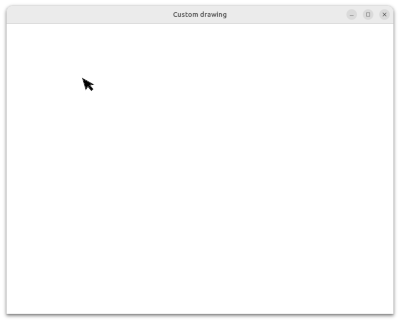
\includegraphics[width=6cm,height=4.83cm]{../image/cd0.png}
\caption{down the button}
\end{figure}

Move the mouse

\begin{figure}
\centering
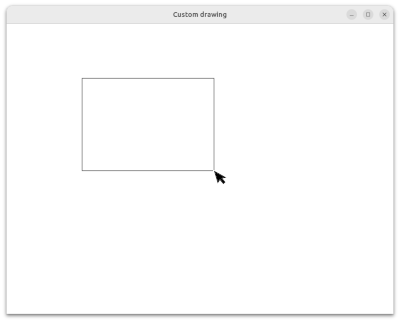
\includegraphics[width=6cm,height=4.83cm]{../image/cd1.png}
\caption{Move the mouse}
\end{figure}

Up the button.

\begin{figure}
\centering
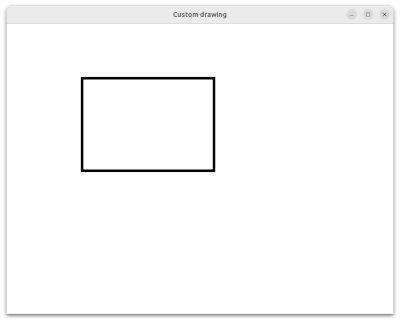
\includegraphics[width=6cm,height=4.83cm]{../image/cd2.png}
\caption{Up the button}
\end{figure}

The programs are at \passthrough{\lstinline!src/custom\_drawing!}
directory. Download the
\href{https://github.com/ToshioCP/Gtk4-tutorial}{repository} and see the
directory. There are four files.

\begin{itemize}
\tightlist
\item
  meson.build
\item
  rect.c
\item
  rect.gresource.xml
\item
  rect.ui
\end{itemize}

\subsection{rect.gresource.xml}\label{rect.gresource.xml}

This file describes a ui file to compile. The compiler
glib-compile-resources uses it.

\begin{lstlisting}[language=XML, numbers=left]
<?xml version="1.0" encoding="UTF-8"?>
<gresources>
  <gresource prefix="/com/github/ToshioCP/rect">
    <file>rect.ui</file>
  </gresource>
</gresources>
\end{lstlisting}

The prefix is \passthrough{\lstinline!/com/github/ToshioCP/rect!} and
the file is \passthrough{\lstinline!rect.ui!}. Therefore, GtkBuilder
reads the resource from
\passthrough{\lstinline!/com/github/ToshioCP/rect/rect.ui!}.

\subsection{rect.ui}\label{rect.ui}

The following is the ui file that defines the widgets. There are two
widgets which are GtkApplicationWindow and GtkDrawingArea. The ids are
\passthrough{\lstinline!win!} and \passthrough{\lstinline!da!}
respectively.

\begin{lstlisting}[language=XML, numbers=left]
<?xml version="1.0" encoding="UTF-8"?>
<interface>
  <object class="GtkApplicationWindow" id="win">
    <property name="default-width">800</property>
    <property name="default-height">600</property>
    <property name="resizable">FALSE</property>
    <property name="title">Custom drawing</property>
    <child>
      <object class="GtkDrawingArea" id="da">
        <property name="hexpand">TRUE</property>
        <property name="vexpand">TRUE</property>
      </object>
    </child>
  </object>
</interface>
\end{lstlisting}

\subsection{rect.c}\label{rect.c}

\subsubsection{GtkApplication}\label{gtkapplication}

This program uses GtkApplication. The application ID is
\passthrough{\lstinline!com.github.ToshioCP.rect!}.

\begin{lstlisting}[language=C]
#define APPLICATION_ID "com.github.ToshioCP.rect"
\end{lstlisting}

See
\href{https://developer.gnome.org/documentation/tutorials/application-id.html}{GNOME
Developer Documentation} for further information.

The function \passthrough{\lstinline!main!} is called at the beginning
of the application.

\begin{lstlisting}[language=C, numbers=left]
int
main (int argc, char **argv) {
  GtkApplication *app;
  int stat;

  app = gtk_application_new (APPLICATION_ID, G_APPLICATION_HANDLES_OPEN);
  g_signal_connect (app, "startup", G_CALLBACK (app_startup), NULL);
  g_signal_connect (app, "activate", G_CALLBACK (app_activate), NULL);
  g_signal_connect (app, "shutdown", G_CALLBACK (app_shutdown), NULL);
  stat =g_application_run (G_APPLICATION (app), argc, argv);
  g_object_unref (app);
  return stat;
}
\end{lstlisting}

It connects three signals and handlers.

\begin{itemize}
\tightlist
\item
  startup: It is emitted after the application is registered to the
  system.
\item
  activate: It is emitted when the application is activated.
\item
  shutdown: It is emitted just before the application quits.
\end{itemize}

\begin{lstlisting}[language=C, numbers=left]
static void
app_startup (GApplication *application) {
  GtkApplication *app = GTK_APPLICATION (application);
  GtkBuilder *build;
  GtkWindow *win;
  GtkDrawingArea *da;
  GtkGesture *drag;

  build = gtk_builder_new_from_resource ("/com/github/ToshioCP/rect/rect.ui");
  win = GTK_WINDOW (gtk_builder_get_object (build, "win"));
  da = GTK_DRAWING_AREA (gtk_builder_get_object (build, "da"));
  gtk_window_set_application (win, app);
  g_object_unref (build);

  gtk_drawing_area_set_draw_func (da, draw_cb, NULL, NULL);
  g_signal_connect_after (da, "resize", G_CALLBACK (resize_cb), NULL);

  drag = gtk_gesture_drag_new ();
  gtk_gesture_single_set_button (GTK_GESTURE_SINGLE (drag), GDK_BUTTON_PRIMARY);
  gtk_widget_add_controller (GTK_WIDGET (da), GTK_EVENT_CONTROLLER (drag));
  g_signal_connect (drag, "drag-begin", G_CALLBACK (drag_begin), NULL);
  g_signal_connect (drag, "drag-update", G_CALLBACK (drag_update), da);
  g_signal_connect (drag, "drag-end", G_CALLBACK (drag_end), da);
}
\end{lstlisting}

The startup handler does three things.

\begin{itemize}
\tightlist
\item
  Builds the widgets.
\item
  Initializes the GtkDrawingArea instance.

  \begin{itemize}
  \tightlist
  \item
    Sets the drawing function
  \item
    Connects the ``resize'' signal and the handler.
  \end{itemize}
\item
  Creates the GtkGestureDrag instance and initializes it. Gesture will
  be explained in this section later.
\end{itemize}

\begin{lstlisting}[language=C, numbers=left]
static void
app_activate (GApplication *application) {
  GtkApplication *app = GTK_APPLICATION (application);
  GtkWindow *win;

  win = gtk_application_get_active_window (app);
  gtk_window_present (win);
}
\end{lstlisting}

The activate handler just shows the window.

\subsubsection{GtkDrawingArea}\label{gtkdrawingarea}

The program has two cairo surfaces and they are pointed by the global
variables.

\begin{lstlisting}[language=C]
static cairo_surface_t *surface = NULL;
static cairo_surface_t *surface_save = NULL;
\end{lstlisting}

The drawing process is as follows.

\begin{itemize}
\tightlist
\item
  Creates an image on \passthrough{\lstinline!surface!}.
\item
  Copies \passthrough{\lstinline!surface!} to the cairo surface of the
  GtkDrawingArea.
\item
  Calls \passthrough{\lstinline!gtk\_widget\_queue\_draw (da)!} to draw
  it if necessary.
\end{itemize}

They are created in the ``resize'' signal handler.

\begin{lstlisting}[language=C, numbers=left]
static void
resize_cb (GtkWidget *widget, int width, int height, gpointer user_data) {
  cairo_t *cr;

  if (surface)
    cairo_surface_destroy (surface);
  surface = cairo_image_surface_create (CAIRO_FORMAT_RGB24, width, height);
  if (surface_save)
    cairo_surface_destroy (surface_save);
  surface_save = cairo_image_surface_create (CAIRO_FORMAT_RGB24, width, height);
  /* Paint the surface white. It is the background color. */
  cr = cairo_create (surface);
  cairo_set_source_rgb (cr, 1.0, 1.0, 1.0);
  cairo_paint (cr);
  cairo_destroy (cr);
}
\end{lstlisting}

This callback is called when the GtkDrawingArea is shown. It is the only
call because the window is not resizable.

It creates image surfaces for \passthrough{\lstinline!surface!} and
\passthrough{\lstinline!surface\_save!}. The
\passthrough{\lstinline!surface!} surface is painted white, which is the
background color.

The drawing function copies \passthrough{\lstinline!surface!} to the
GtkDrawingArea surface.

\begin{lstlisting}[language=C, numbers=left]
static void
draw_cb (GtkDrawingArea *da, cairo_t *cr, int width, int height, gpointer user_data) {
  if (surface) {
    cairo_set_source_surface (cr, surface, 0.0, 0.0);
    cairo_paint (cr);
  }
}
\end{lstlisting}

This function is called by the system when it needs to redraw the
drawing area.

Two surfaces \passthrough{\lstinline!surface!} and
\passthrough{\lstinline!surface\_save!} are destroyed before the
application quits.

\begin{lstlisting}[language=C, numbers=left]
static void
app_shutdown (GApplication *application) {
  if (surface)
    cairo_surface_destroy (surface);
  if (surface_save)
    cairo_surface_destroy (surface_save);
}
\end{lstlisting}

\subsubsection{GtkGestureDrag}\label{gtkgesturedrag}

Gesture class is used to recognize human gestures such as click, drag,
pan, swipe and so on. It is a subclass of GtkEventController. GtkGesture
class is abstract and there are several implementations.

\begin{itemize}
\tightlist
\item
  GtkGestureClick
\item
  GtkGestureDrag
\item
  GtkGesturePan
\item
  GtkGestureSwipe
\item
  other implementations
\end{itemize}

The program \passthrough{\lstinline!rect.c!} uses GtkGestureDrag. It is
the implementation for drags. The parent-child relationship is as
follows.

\begin{lstlisting}
GObject -- GtkEventController -- GtkGesture -- GtkGestureSingle -- GtkGestureDrag
\end{lstlisting}

GtkGestureSingle is a subclass of GtkGesture and optimized for
singe-touch and mouse gestures.

A GtkGestureDrag instance is created and initialized in the startup
signal handler in \passthrough{\lstinline!rect.c!}. See line 18 to 23 in
the following.

\begin{lstlisting}[language=C, numbers=left]
static void
app_startup (GApplication *application) {
  GtkApplication *app = GTK_APPLICATION (application);
  GtkBuilder *build;
  GtkWindow *win;
  GtkDrawingArea *da;
  GtkGesture *drag;

  build = gtk_builder_new_from_resource ("/com/github/ToshioCP/rect/rect.ui");
  win = GTK_WINDOW (gtk_builder_get_object (build, "win"));
  da = GTK_DRAWING_AREA (gtk_builder_get_object (build, "da"));
  gtk_window_set_application (win, app);
  g_object_unref (build);

  gtk_drawing_area_set_draw_func (da, draw_cb, NULL, NULL);
  g_signal_connect_after (da, "resize", G_CALLBACK (resize_cb), NULL);

  drag = gtk_gesture_drag_new ();
  gtk_gesture_single_set_button (GTK_GESTURE_SINGLE (drag), GDK_BUTTON_PRIMARY);
  gtk_widget_add_controller (GTK_WIDGET (da), GTK_EVENT_CONTROLLER (drag));
  g_signal_connect (drag, "drag-begin", G_CALLBACK (drag_begin), NULL);
  g_signal_connect (drag, "drag-update", G_CALLBACK (drag_update), da);
  g_signal_connect (drag, "drag-end", G_CALLBACK (drag_end), da);
}
\end{lstlisting}

\begin{itemize}
\tightlist
\item
  The function \passthrough{\lstinline!gtk\_gesture\_drag\_new!} creates
  a new GtkGestureDrag instance.
\item
  The function
  \passthrough{\lstinline!gtk\_gesture\_single\_set\_button!} sets the
  button number to listen to. The constant
  \passthrough{\lstinline!GDK\_BUTTON\_PRIMARY!} is the left button of a
  mouse.
\item
  The function \passthrough{\lstinline!gtk\_widget\_add\_controller!}
  adds an event controller, gestures are descendants of the event
  controller, to a widget.
\item
  Three signals and handlers are connected.

  \begin{itemize}
  \tightlist
  \item
    drag-begin: Emitted when dragging starts.
  \item
    drag-update: Emitted when the dragging point moves.
  \item
    drag-end: Emitted when the dragging ends.
  \end{itemize}
\end{itemize}

The process during the drag is as follows.

\begin{itemize}
\tightlist
\item
  start: save the surface and start points
\item
  update: restore the surface and draw a thin rectangle between the
  start point and the current point of the mouse
\item
  end: restore the surface and draw a thick rectangle between the start
  and end points.
\end{itemize}

We need two global variables for the start point.

\begin{lstlisting}[language=C]
static double start_x;
static double start_y;
\end{lstlisting}

The following is the handler for the ``drag-begin'' signal.

\begin{lstlisting}[language=C, numbers=left]
static void
copy_surface (cairo_surface_t *src, cairo_surface_t *dst) {
  if (!src || !dst)
    return;
  cairo_t *cr = cairo_create (dst);
  cairo_set_source_surface (cr, src, 0.0, 0.0);
  cairo_paint (cr);
  cairo_destroy (cr);
}

static void
drag_begin (GtkGestureDrag *gesture, double x, double y, gpointer user_data) {
  // save the surface and record (x, y)
  copy_surface (surface, surface_save);
  start_x = x;
  start_y = y;
}
\end{lstlisting}

\begin{itemize}
\tightlist
\item
  Copies \passthrough{\lstinline!surface!} to
  \passthrough{\lstinline!surface\_save!}, which is an image just before
  the dragging.
\item
  Stores the points to \passthrough{\lstinline!start\_x!} and
  \passthrough{\lstinline!start\_y!}.
\end{itemize}

\begin{lstlisting}[language=C, numbers=left]
static void
drag_update  (GtkGestureDrag *gesture, double offset_x, double offset_y, gpointer user_data) {
  GtkWidget *da = GTK_WIDGET (user_data);
  cairo_t *cr;
  
  copy_surface (surface_save, surface);
  cr = cairo_create (surface);
  cairo_rectangle (cr, start_x, start_y, offset_x, offset_y);
  cairo_set_line_width (cr, 1.0);
  cairo_stroke (cr);
  cairo_destroy (cr);
  gtk_widget_queue_draw (da);
}
\end{lstlisting}

\begin{itemize}
\tightlist
\item
  Restores \passthrough{\lstinline!surface!} from
  \passthrough{\lstinline!surface\_save!}.
\item
  Draws a rectangle with thin lines.
\item
  Calls \passthrough{\lstinline!gtk\_widget\_queue\_draw!} to add the
  GtkDrawingArea to the queue to redraw.
\end{itemize}

\begin{lstlisting}[language=C, numbers=left]
static void
drag_end  (GtkGestureDrag *gesture, double offset_x, double offset_y, gpointer user_data) {
  GtkWidget *da = GTK_WIDGET (user_data);
  cairo_t *cr;
  
  copy_surface (surface_save, surface);
  cr = cairo_create (surface);
  cairo_rectangle (cr, start_x, start_y, offset_x, offset_y);
  cairo_set_line_width (cr, 6.0);
  cairo_stroke (cr);
  cairo_destroy (cr);
  gtk_widget_queue_draw (da);
}
\end{lstlisting}

\begin{itemize}
\tightlist
\item
  Restores \passthrough{\lstinline!surface!} from
  \passthrough{\lstinline!surface\_save!}.
\item
  Draws a rectangle with thick lines.
\item
  Calls \passthrough{\lstinline!gtk\_widget\_queue\_draw!} to add the
  GtkDrawingArea to the queue to redraw.
\end{itemize}

\subsection{Build and run}\label{build-and-run}

Download the
\href{https://github.com/ToshioCP/Gtk4-tutorial}{repository}. Change
your current directory to \passthrough{\lstinline!src/custom\_drawing!}.
Run meson and ninja to build the program. Type
\passthrough{\lstinline!\_build/rect!} to run the program. Try to draw
rectangles.

\begin{lstlisting}
$ cd src/custom_drawing
$ meson setup _build
$ ninja -C _build
$ _build/rect
\end{lstlisting}

\begin{figure}
\centering
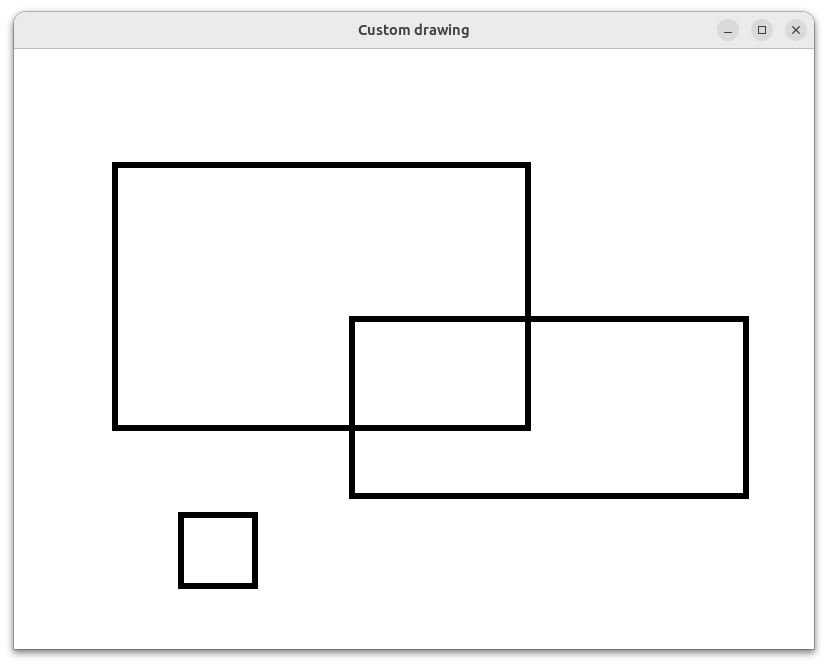
\includegraphics[width=12.4cm,height=10cm]{../image/rect.png}
\caption{The screen of rect program}
\end{figure}
